\documentclass[boxes]{homework}

% This is a slightly-more-than-minimal document that uses the homework class.
% See the README at http://git.io/vZWL0 for complete documentation.

\name{傅申 PB20000051}        % Replace (Your Name) with your name.
\term{2022 秋}     % Replace (Current Term) with the current term.
\course{算法基础}    % Replace (Course Name) with the course name.
\hwnum{3}          % Replace (Number) with the number of the homework.
\hwname{作业}
\problemname{}
\solutionname{解:}

% Load any other packages you need here.
\usepackage[
    a4paper,
    top = 2.54cm,
    bottom = 2.54cm,
    left = 1.91cm,
    right = 1.91cm,
    includeheadfoot
]{geometry}
\fancyfootoffset{0pt} % make fancyhdr work properly
\usepackage{ctex}
\usepackage{tikz}
\usepackage{subcaption}
\tikzset{
    node distance=1cm,
    every node/.style={circle, draw, minimum size=0.8cm},
    current/.style={fill=gray},
    level/.style={sibling distance=4cm/#1, level distance=1cm},
    level 3/.style={sibling distance=1cm, level distance=1cm},
}

\begin{document}
%%%% Problem 6.1-3 %%%%
\problemchap{6}
\problempart{1}
\problemnumber{3}
\begin{problem}
证明: 在最大堆的任一子树中, 该子树所包含的最大元素在该子树的根结点上.
\end{problem}
\begin{solution}
    采用反证法, 假设该子树所包含的最大元素 $A[i]$ 不在该子树的根结点上, 则最大元
    素的父亲也在该子树中, 有 $A[\operatorname{PARENT}(i)] < A[i]$, 不满足最大堆
    性质, 矛盾. 因此该子树所包含的最大元素在该子树的根结点上.
\end{solution}

%%%% Problem 6.1-5 %%%%
\problemnumber{5}
\begin{problem}
一个已排好序的数组是一个最小堆吗?
\end{problem}
\begin{solution}
    因为 $\operatorname{PARENT}(i) = \lfloor i / 2 \rfloor \leqslant i$, 所以对
    一个已排好序的数组, 除了根以外的结点 $i$ 都有
    $A[\operatorname{PARENT}(i)] \leqslant A[i]$, 满足最小堆性质. 因此一个已排好
    序的数组是一个最小堆.
\end{solution}

%%%% Problem 6.2-3 %%%%
\problempart{2}
\problemnumber{3}
\begin{problem}
当元素 $A[i]$ 比其孩子的值都大时, 调用 MAX-HEAPIFY ($A$, $i$) 会有什么结果?
\end{problem}
\begin{solution}
    在第 7 行结束后, $largest = i$, 不会进入第 8 行的 \textbf{if} 语句, 直接结束
    运行而不改变任何元素.
\end{solution}

%%%% Problem 6.2-5 %%%%
\problemnumber{5}
\begin{problem}
MAX-HEAPIFY 的代码效率很高, 但第 10 行中的递归调用可能例外, 它可能使某些编译器产
生低效的代码. 请用循环控制结构取代递归, 重写 MAX-HEAPIFY 代码.
\end{problem}
\begin{solution}
    如下
    \begin{algo}
        \caption{LOOP-MAX-HEAPIFY ($A$, $i$)}
        \label{algo:1}
        \While{$i \leqslant A.heap\text{-}size$}{
            $l = \operatorname{LEFT}(i)$\;
            $r = \operatorname{RIGHT}(i)$\;
            \eIf{$l\leqslant A.heap\text{-}size$ and $A[l] > A[i]$}{
                $largest = l$\;
            }{
                $largest = i$\;
            }
            \If{$r\leqslant A.heap\text{-}size$ and $A[r] > A[i]$}{
                $largest = r$\;
            }
            \If{$largest = i$}{
                \textbf{break}\;
            }
            exchange $A[i]$ with $A[largest]$\;
            $i = largest$\;
        }
    \end{algo}
\end{solution}

%%%% Problem 6.3-3 %%%%
\problempart{3}
\problemnumber{3}
\begin{problem}
证明: 对于任一包含 $n$ 个元素的堆中, 至多有 $\left\lceil n / 2^{h + 1}
    \right\rceil$ 个高度为 $h$ 的结点.
\end{problem}
\begin{solution}
    记高度为 $h$ 的结点有 $n_{h}$ 个. 使用数学归纳法, 先考虑 $n_{0}$. 因为高度为
    0 的结点就是叶节点, 而堆中叶节点的个数为 $\lceil n / 2 \rceil$, 所以满足
    \begin{equation}
        n_{0} \leqslant \left\lceil n / 2^{0 + 1} \right\rceil
    \end{equation}
    现在假设 $n_{h - 1}$ 满足 $n_{h - 1} \leqslant \left\lceil n / 2^{(h - 1)+1}
        \right\rceil$, 则对于 $n_{h}$, 若 $n_{h - 1}$ 为偶数, 则 $n_{h} =
        n_{h - 1} / 2 = \left\lceil n_{h - 1} / 2 \right\rceil$; 若 $n_{h - 1}$
    为奇数, 则 $n_{h} = \left\lfloor n_{h - 1} / 2 \right\rfloor + 1 =
        \left\lceil n_{h - 1} / 2 \right\rceil$. 因此
    \begin{equation}
        n_{h} = \left\lceil \frac{ n_{h - 1} }{ 2 } \right\rceil
        \leqslant \left\lceil \frac{ \left\lceil n / 2^{(h - 1) + 1} \right\rceil }
        { 2 } \right\rceil
        = \left\lceil n / 2^{h + 1} \right\rceil
    \end{equation}
    所以对所有的 $h$, 至多有 $\left\lceil n / 2^{h + 1}\right\rceil$ 个高度为
    $h$ 的结点.
\end{solution}

%%%% Problem 6.4-4 %%%%
\problempart{4}
\problemnumber{4}
\begin{problem}
证明: 在最坏情况下, HEAPSORT 的时间复杂度是 $\Omega(n\lg n)$.
\end{problem}
\begin{solution}
    先只考虑 HEAPSORT 的循环部分, 若每次调用 MAX-HEAPIFY 都要将根结点逐步交换到
    最低的结点 (比如每次都交换到 $A[A.heap\text{-}size]$), 则出现最坏情况, 比如
    输入数组已降序排序好. 在这种情况下, 每次每次调用 MAX-HEAPIFY 都要花费
    $\Theta  \left( \lfloor \lg i \rfloor\right)$ 的时间, 所以循环部分的时间复
    杂度为
    \begin{equation}
        \sum_{i = n}^{2} \Theta \left( \lfloor \lg i \rfloor \right) + \Theta(1)
        = \Theta \left( \lg n! + n\right)
        = \Theta \left( n \lg n\right)
    \end{equation}
    而 BUILD-MAX-HEAP 的时间复杂度为 $O(n)$, 所以最坏情况下 HEAPSORT 的时间复杂
    度满足 $T(n) = \Theta(n\lg n) + O(n)$, 显然有下界 $\Omega(n\lg n)$.
\end{solution}

%%%% Problem 6.5-2 %%%%
\problempart{5}
\problemnumber{2}
\begin{problem}
试说明 MAX-HEAP-INSERT ($A$, 10) 在堆 $A = \left\langle 15, 13, 9, 5, 12,
    8, 7, 4, 0, 6, 2, 1\right\rangle$ 上的操作过程.
\end{problem}
\begin{solution}
    如图~\ref{fig:6.5-2} 所示.
    \begin{figure}[ht]
        \centering
        \begin{subfigure}[ht]{0.4\textwidth}
            \centering
            \resizebox{\textwidth}{!}{
                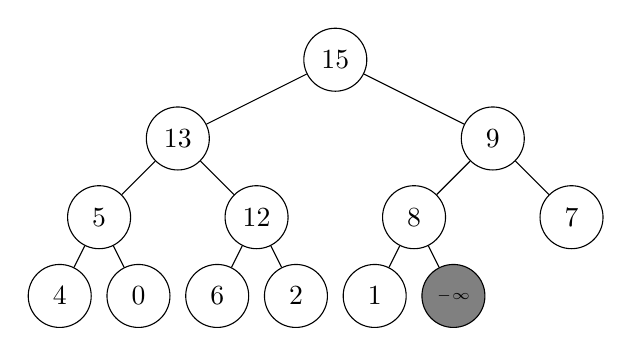
\begin{tikzpicture}
                    \node {15}
                    child{node {13}
                            child {node {5}
                                    child {node {4}}
                                    child {node {0}}
                                }
                            child {node {12}
                                    child {node {6}}
                                    child {node {2}}
                                }
                        }
                    child{node {9}
                            child{node {8}
                                    child{node {1}}
                                    child{node[current] {\tiny $- \infty$}}
                                }
                            child{node {7}}
                        };
                \end{tikzpicture}
            }
            \caption{}
        \end{subfigure}
        \begin{subfigure}[ht]{0.4\textwidth}
            \centering
            \resizebox{\textwidth}{!}{
                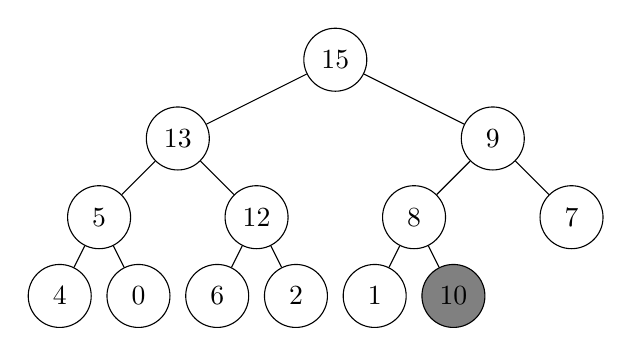
\begin{tikzpicture}
                    \node {15}
                    child{node {13}
                            child {node {5}
                                    child {node {4}}
                                    child {node {0}}
                                }
                            child {node {12}
                                    child {node {6}}
                                    child {node {2}}
                                }
                        }
                    child{node {9}
                            child{node {8}
                                    child{node {1}}
                                    child{node[current] {10}}
                                }
                            child{node {7}}
                        };
                \end{tikzpicture}
            }
            \caption{}
        \end{subfigure}
        \begin{subfigure}[ht]{0.4\textwidth}
            \centering
            \resizebox{\textwidth}{!}{
                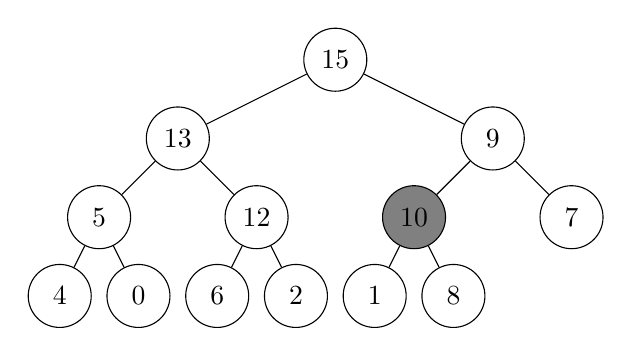
\begin{tikzpicture}
                    \node {15}
                    child{node {13}
                            child {node {5}
                                    child {node {4}}
                                    child {node {0}}
                                }
                            child {node {12}
                                    child {node {6}}
                                    child {node {2}}
                                }
                        }
                    child{node {9}
                            child{node[current] {10}
                                    child{node {1}}
                                    child{node {8}}
                                }
                            child{node {7}}
                        };
                \end{tikzpicture}
            }
            \caption{}
        \end{subfigure}
        \begin{subfigure}[ht]{0.4\textwidth}
            \centering
            \resizebox{\textwidth}{!}{
                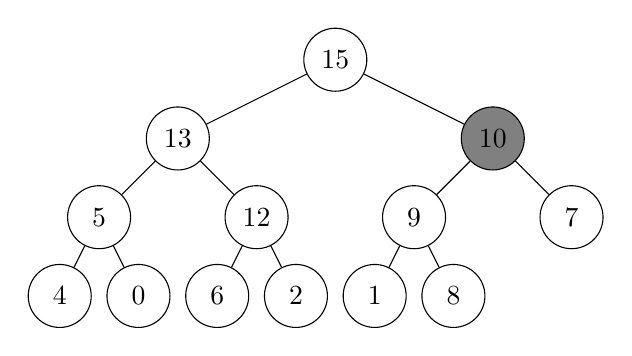
\begin{tikzpicture}
                    \node {15}
                    child{node {13}
                            child {node {5}
                                    child {node {4}}
                                    child {node {0}}
                                }
                            child {node {12}
                                    child {node {6}}
                                    child {node {2}}
                                }
                        }
                    child{node[current] {10}
                            child{node {9}
                                    child{node {1}}
                                    child{node {8}}
                                }
                            child{node {7}}
                        };
                \end{tikzpicture}
            }
            \caption{}
        \end{subfigure}
        \caption{MAX-HEAP-INSERT($A$, 10) 的操作过程}
        \label{fig:6.5-2}
    \end{figure}
\end{solution}

%%%% Problem 6.5-4 %%%%
\problemnumber{4}
\begin{problem}
在 MAX-HEAP-INSERT 的第 2 行, 为什么我们要先把关键字设为 $-\infty$, 然后又将其增
加到需要的值呢?
\end{problem}
\begin{solution}
    先将关键字设为 $-\infty$ 能保证调用 HEAP-INCREASE-KEY 时, 输入的数组满足最大
    堆性质, 是一个最大堆.
\end{solution}

%%%% Problem 7.2-2 %%%%
\problemchap{7}
\problempart{2}
\problemnumber{2}
\begin{problem}
当数组 $A$ 的所有元素都具有相同值时, QUICKSORT 的时间复杂度是什么?
\end{problem}
\begin{solution}
    所有元素都具有相同值时, PARTITION 会将数组分为长度为 0 和 $n - 1$ 的两个子数
    组, 即最坏情况, 时间复杂度为 $\Theta \left( n^{2}\right)$.
\end{solution}

%%%% Problem 7.2-5 %%%%
\problemnumber{5}
\begin{problem}
假设快速排序每一层所做的划分的比例都是 $1 - \alpha : \alpha$, 其中
$0 < \alpha \leqslant 1 / 2$ 且是一个常数. 试证明: 在相应递归树中, 叶节点的最小
深度大约是 $- \lg n / \lg a$, 最大深度大约是 $- \lg n / \lg (1 - \alpha)$.
(无需考虑整数舍入问题).
\end{problem}
\begin{solution}
    递归树深度最小的叶结点对应每次都取较小的子问题, 即取长度比例为 $\alpha$ 的子
    数组, 就有 $1 \approx \alpha^{k}n \Rightarrow k \approx  \log_{\alpha}
        \dfrac{ 1 }{ n } = -\lg n / \lg a$. 同理, 递归树深度最大的叶结点对应每次
    都取较大的子问题, 即取长度比例为 $1 - \alpha$ 的子数组, 就有 $1 \approx
        (1 - \alpha)^{k}n \Rightarrow k \approx  \log_{1 - \alpha}
        \dfrac{ 1 }{ n } = -\lg n / \lg (1 - \alpha)$.
\end{solution}

%%%% Problem 7.4-5 %%%%
\problempart{4}
\problemnumber{5}
\begin{problem}
当输入数据已经 ``几乎有序'' 时, 插入排序速度很快. 在实际应用中, 我们可以利用这一
特点来提高快速排序的速度. 当对一个长度小于 $k$ 的子数组调用快速排序时, 让它不做
任何排序就返回. 当上层的快速排序调用返回后, 对整个数组运行插入排序来完成排序过
程. 试证明: 这一排序算法的期望时间复杂度为 $O (nk + n\lg (n / k))$. 分别从理论
和实践的角度说明我们应该如何选择 $k$?
\end{problem}
\begin{solution}
    因为修改后的快速排序在对长度小于 $k$ 的子数组不作操作就返回, 因此递归树的高
    度将减小 $\lg k$, 对应期望时间复杂度为 $O(n (\lg n-\lg k)) = O(n\lg (n/k))$.
    而插入排序对快速排序返回的数组排序时, 等价于分别对 $n / k$ 个长度为 $k$ 的子
    数组进行插入排序, 对应时间复杂度为 $n O(k^{2})/k = O(nk)$. 因此, 总的时间复
    杂度为 $O(nk + n\lg (n / k))$.

    从理论的角度, 要让 $nk + n\lg (n / k)$ 尽可能小. 对 $k$ 取导数得到
    $n (1 - 1 / k\ln 2) = 0$, 取 $k = 1 / \ln 2$ 时能得到最小值. 从实践的角度,
    排序算法的快慢不仅需要考虑复杂度, 还要考虑存储层次等其他因素, 因此 $k$ 的选
    取需要经过实验确定.
\end{solution}

%%%% Problem 8.1-4 %%%%
\problemchap{8}
\problempart{1}
\problemnumber{4}
\begin{problem}
假设现有一个包含 $n$ 个元素的待排序序列. 该序列由 $n / k$ 个子序列组成, 每个子序
列包含 $k$ 个元素. 一个给定子序列中的每个元素都小于其后继子序列中的所有元素, 且
大于其前驱子序列中的所有元素. 因此, 对于这个长度为 $n$ 的序列的排序转化为对
$n / k$ 个子序列的 $k$ 个元素的排序. 试证明: 这个排序问题中所需比较次数的下界是
$\Omega(n\lg k)$. (\emph{提示:} 简单地将每个子序列的下界进行合并是不严谨的.)
\end{problem}
\begin{solution}
    输入数据可能的排列数有 ${\left( k !\right)}^{n / k}$ 种, 因此一个比较排序算法
    的比较次数 $h$ 满足
    \begin{equation}
        {\left( k!\right)}^{n / k} \leqslant 2^{h} \Rightarrow
        h \geqslant \frac{ n }{ k } \lg k! = \frac{ n }{ k } \Omega(k \lg k)
        = \Omega(n \lg k)
    \end{equation}
\end{solution}

\end{document}
